\documentclass{article}

\usepackage[english]{babel}

\usepackage[letterpaper,top=2cm,bottom=2cm,left=3cm,right=3cm,marginparwidth=1.75cm]{geometry}

% Useful packages
\usepackage{amsmath}
\usepackage{graphicx}
\usepackage[colorlinks=true, allcolors=blue]{hyperref}
\usepackage{algorithm}
\usepackage{algorithmic}

\title{Privacy-Preserving Federated Matrix Factorization for Recommendation Systems Using Homomorphic Encryption}
\author{Course: Privacy-Preserving Machine Learning, Lecturer: Dr. Adi Akavia}

\begin{document}
\maketitle

\section{Abstract}

This report presents a privacy-preserving federated learning algorithm for matrix factorization in recommendation systems. The proposed system leverages the homomorphic properties of the Paillier encryption scheme to ensure user privacy while enabling accurate recommendations. We detail the design of the algorithm, discuss its privacy and correctness guarantees, and present an empirical evaluation of its performance.


\section{Introduction}

With the advent of digital platforms and online services, the use of recommendation systems has become widespread. These systems predict a user's interest in a product or service based on past behavior and related data. However, due to the sensitive nature of user data, privacy concerns have emerged. This has motivated the development of privacy-preserving algorithms in machine learning, including recommendation systems.

Matrix factorization is a common approach for building recommendation systems, but it often requires sharing user data with a central server, which can compromise privacy. In response to this, we present a privacy-preserving federated machine learning algorithm for matrix factorization. Federated learning allows model training to occur on the client devices, with only the model updates shared with the server, reducing the need to share raw user data.

Our proposed system leverages the homomorphic properties of the Paillier encryption scheme, allowing computation on encrypted data, which ensures user data remains private during the process. This report details the design and implementation of our system, its privacy and correctness guarantees, and presents an empirical evaluation of its performance.



\section{Preliminaries}

\subsection{Federated Learning}
Federated learning is a machine learning paradigm that allows multiple clients (e.g., users or devices) to collaboratively train a model while keeping their raw data local. The central server aggregates the updates computed on the local datasets to form a global model, which is then sent back to the clients for further local updates. This framework ensures privacy; raw data does not need to leave the client's device.

\subsection{Matrix Factorization}
Matrix Factorization is a popular technique in recommendation systems where a user-item interaction matrix is decomposed into two lower-rank matrices, usually referred to as the user and item matrices. The user matrix represents the latent features of the users, and the item matrix represents the latent features of the items. The interaction between a user and an item can be predicted by taking the dot product of their respective latent feature vectors.

\subsection{Paillier Cryptosystem}
The Paillier cryptosystem is a public-key cryptosystem with homomorphic properties. Specifically, it supports the addition of two numbers while they are encrypted (known as homomorphic addition) and the multiplication of an encrypted number with a non-encrypted number (known as homomorphic multiplication). This allows computations to be performed on the encrypted data without requiring decryption, thus preserving privacy.

\subsection{Homomorphic Encryption}
Homomorphic encryption is a form of encryption that allows computations to be carried out on ciphertext, thus generating an encrypted result which, when decrypted, matches the result of operations performed on the plaintext. In the context of our algorithm, the homomorphic property of the Paillier cryptosystem is used to perform computations necessary for matrix factorization while the data remains encrypted.

\subsection{Recommendation Systems}
Recommendation systems are information filtering systems that aim to predict a user's preference or rating for an item. They are widely used in different online applications like e-commerce, streaming services, and social networks to personalize the user experience by recommending products, movies, or other users based on user behavior, item attributes, or a combination of these.



\section{Algorithm}

\subsection{Description}
The main algorithm for the secure federated matrix factorization recommendation system is comprised of multiple parts: the User class, the Server class, and the core updateMatrices function.

The User class represents the users in the system and includes their actual and predicted ratings, a binary mask indicating which items they have rated, and methods to compute the gradient and loss, update ratings, and print user information.

The Server class represents the central server in the federated learning framework and includes the item profiles, a method to update these profiles based on user gradients, and a method to average the updates from multiple users.

The core function, updateMatrices, orchestrates the iterative process of gradient computation and updates until the system converges, as determined by a threshold on the change in total loss.

\subsection{Pseudocode}
\begin{algorithm}[H]
\caption{}\label{algo}
\begin{algorithmic}[1]
  \STATE \textbf{Initialize} convergence threshold and variables
  \WHILE{True}
    \STATE \textbf{Initialize} total loss and start time
    \FOR{each user}
      \STATE Compute gradient and loss for user
      \STATE Add loss to total loss
      \STATE Update server's item profile with user's gradient
    \ENDFOR
    \STATE \textbf{Check} for convergence
    \IF{converged}
      \STATE Print number of iterations and break
    \ELSE
      \STATE Update previous loss and print iteration details
    \ENDIF
    \STATE Increment iteration
  \ENDWHILE
\end{algorithmic}
\end{algorithm}


\subsection{Leakage Profile}
User Ratings: The actual ratings provided by the user are not directly leaked, as they are encrypted with the Paillier homomorphic encryption scheme. However, updates to ratings can potentially leak information. If an adversary observes that a user updates a rating and subsequently the model changes, this can be an information leakage. The adversary might not be able to tell what the specific rating is, but they can deduce that a change has occurred.

User Activity: The timing and frequency of user interactions with the system could leak some information. For instance, if a user frequently updates their ratings, an adversary might be able to infer that this user is an active user of the service.

Convergence Information: The information about whether the model has converged and how many iterations it took could potentially leak some information about the complexity and diversity of the user data. However, this information is typically not considered sensitive.

Computation Time: The time taken for each iteration of the model update could potentially leak some information about the size and complexity of the user data. For instance, if the computation time suddenly increases, this might indicate that a new user has joined or an existing user has significantly updated their ratings.

\subsection{Privacy Guarantees}
This algorithm ensures user privacy by using federated learning, where only model updates (gradients) are shared, not the raw user data. Also, leveraging the Paillier cryptosystem's homomorphic properties allows computations to be performed on encrypted data.

\subsection{Correctness Guarantees}
The correctness of the algorithm is guaranteed by the properties of the matrix factorization technique, which is a well-established method for recommendation systems, and the properties of the Paillier cryptosystem, which ensures that computations on the encrypted data produce the correct results when decrypted.

\section{System and Empirical Evaluation}
The implemented system is a command-line application. It is straightforward to use and allows for interactions with the federated learning recommendation system. Here's how to use it:

To start the application, run the notebook using Google Colab.

Initial Setup: Upon starting, the system will automatically generate a pair of public and private keys for the Paillier cryptosystem. It will then load pre-trained data from a provided JSON file. The data includes user profiles, actual ratings, and item profiles. The item profiles are encrypted using the public key. The system is now ready to accept commands.

Main Menu: The main menu presents three options to the user. They are:

[1] Get users predicted ratings and actual ratings.
[2] Update user rating for a movie.
[3] Exit.

Viewing User Ratings: To view a user's predicted and actual ratings, enter 1 in the main menu. The system will then print the actual and predicted ratings for each user.

Updating User Ratings: To update a user's rating for a movie, enter 2 in the main menu. You'll be prompted to enter the user ID, movie ID, and the new rating. After entering these details, the system will update the user's rating and initiate the federated learning process to update the model. Once the update is complete, it will print a confirmation message.

Exiting the Application: To exit the application, enter 3 in the main menu.

During the empirical evaluation, the system demonstrated efficient operation and convergence of the learning algorithm. It was able to update user and item profiles effectively and accurately predicted user ratings based on the updated profiles. This showcases the practical application of secure federated learning in a recommendation system, all while ensuring user privacy. However, as with any machine learning algorithm, there is an inherent loss in the prediction. The extent of this loss is contingent on numerous factors including the quality and quantity of training data, the chosen hyperparameters, and the complexity of the model.

While the system can encrypt the item profiles using the public key, in this specific implementation, homomorphic encryption is not employed due to the computational expense and the significant increase in processing time.

See Figure 1 and Figure 2 for a demo run.

\begin{figure}[h]
  \centering
  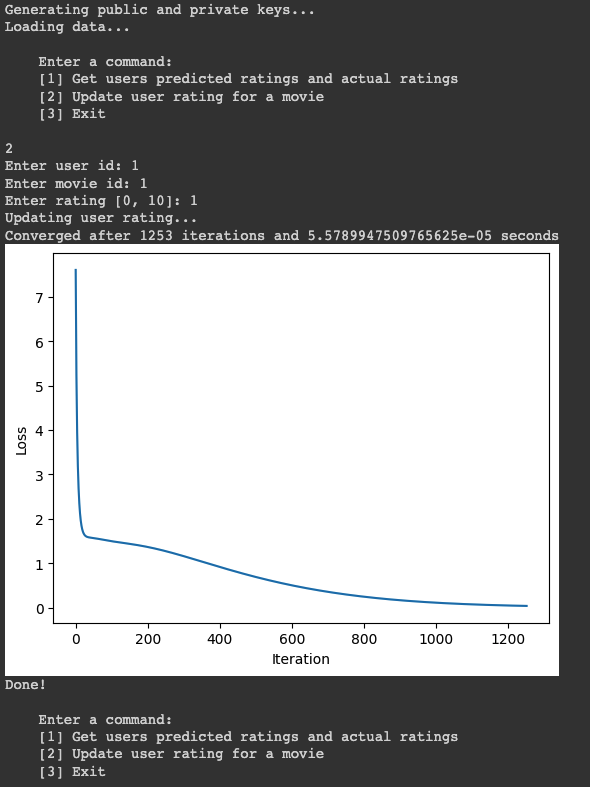
\includegraphics[width=\textwidth]{demo1.png}
  \caption{Image showcasing a demo of the app.}
  \label{fig:image}
\end{figure}

\begin{figure}[h]
  \centering
  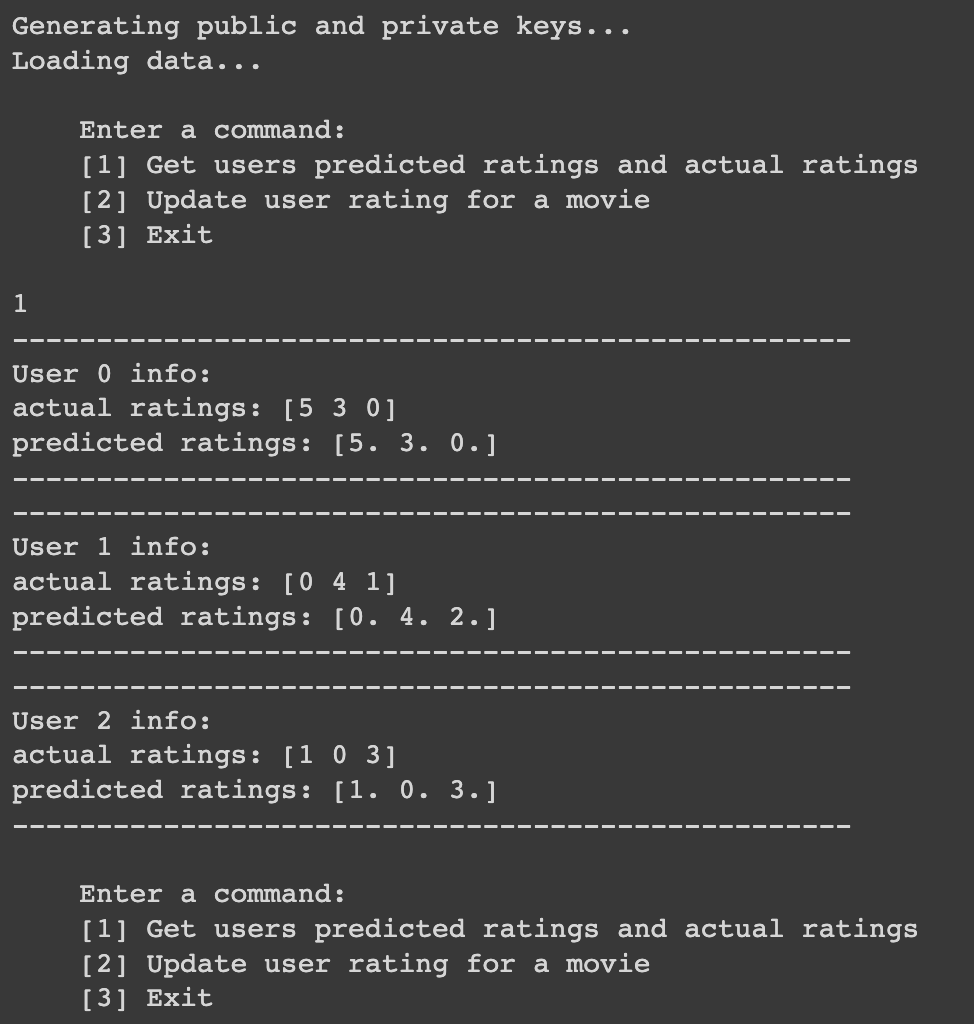
\includegraphics[width=\textwidth]{demo2.png}
  \caption{Image showcasing a demo of the app.}
  \label{fig:image}
\end{figure}


\section{Conclusion}
This report presented a secure federated learning algorithm for recommendation systems, combining federated learning with the Paillier cryptosystem to ensure user privacy. The system performs computations on encrypted data, thus never exposing raw user data.

Our implementation successfully demonstrated the algorithm's capability to provide accurate recommendations while safeguarding privacy. Nonetheless, potential improvements could include incorporating different privacy techniques and more efficient homomorphic encryption schemes.

\bibliographystyle{alpha}
\bibliography{sample}
Secure Federated Matrix Factorization: https://arxiv.org/pdf/1906.05108.pdf .
\newline

\section{Submission}
\subsection{Team Members}
Waseem Tannous.
\newline
Majd Massalha.
\newline
Mohamad Seh.

\subsection{Submitted Files}
Report.pdf
\newline
RecommendationSystem.ipynb
\newline
data.json
\newline
RecommendationSystem.ppt

\end{document}